
\section{Project Documentation}

	\begin{displayquote}
	"You're growing, learning so quickly. I am frightened of what you might become, what path you might take."
	-Bernard Lowe, \textit{Westworld, Season 2 Episode 1}
	\end{displayquote}

\subsection{Summary of Project}
Our project is named "How to make an Effective Robot Comedian."
\textit{Effective} is a quality that establishes the comedic devices that work best for a specific audience.
The robot that we used was a NAO, from Softbank Robotics. We referred to it as "Ginger."
Ginger was a gentle, yet clumsy Robot that was new to the world around her.
She has tried many things before becoming a Robot Comedian, and has a few stories (jokes) about her experience in a human world.
This section will cover our Comedy Show that we had Ginger perform, and how our research categories affected the show.


\subsection{Theory of Writing Jokes}
A joke is setting up an expectation, and then breaking that expectation.
A joke can be subjectively funny to the comedian; the only way to find what is funny to an audience is telling that audience the joke.
Each joke followed a simple structure, \textit{\textbf{Setup, Premise, and Punch}}.

    \begin{enumerate}
        \item{\textbf{Setup}}

            The Setup "mounts", a joke, and leads the monologue the comedian is having towards a specific topic.


            Ex: "I tried being an autonomous car recently, it did not go well."
        \item{\textbf{Premise}}

            The premise is what establishes the expectation of the topic in the setup.


            Ex: "I hit an old woman with my car, and she landed on my hood"
        \item{\textbf{Punch}}

            The punch is what breaks the expectation established during the premise.


            Ex: "So I decided to take her where she wanted to go. She did not even say 'Thank You'".
            We thought that this was funny because Ginger claims it did not go well only because the old woman (which she hit) did not say 'Thanks.'
    \end{enumerate}

This model can be applied many different ways.
We often had a setup we though could be funny, and then filled in the premise and punch to see what was most effective.
You can also think of a premise, and then write a punch and setup that fits the premise.
You can also think of a punch, and then write a premise and setup that fits the punch.

We found that the best comedic device (common setup) for Ginger was \textit{Self-Depreciation}.
Ginger did not move like a human, even though she was a humanoid robot.
So we thought it would be funny if she couldn't figure out why she didn't understand things.
Whenever she moved in a way that was unexpected and not human, people thought it was a funny bit.

\subsection{Research Categories}

    During this project, we spent time researching three different aspects of robot comedy.
    This is the order in which we think Robot Comedy is most effective:

		\begin{enumerate}
			\item{Crowd Work}
			\item{Robot VS Human Character}
			\item{Performance Adaptation}
		\end{enumerate}

    %\subsubsection{Crowd Work}
    %\subsubsection{Robot VS Human Character}
    %\subsubsection{Performance Adaptation}
        The performance branched depending on what the crowd chose for a topic, either "Jobs, Romance, or Aging."
        We had the crowd make some noise for the topic they would like to hear.
        Out of the 9 shows that we performed at Expo, 8 of the shows picked the last topic.
        This method of branching is not advised, as the crowd should not be in control of the show ("See 'Designing a Performance'").

        We collected audio information for each behavior, and then averaged the result to get an "average response" for the show.
        This did not result in a better show. It is more effective to design 1 show, instead of the three (between the three topics).
        Most people only saw the show once, and these crowds saw "Aging", as it was a choice that was presented last.
        It was hard to tell if the audience was intentionally choosing "Aging", or if they cheered for the last response so that their response was chosen.

\subsection{Animating the NAO}
Animating the NAO robot could be done virtually, and hands-on.
Animations are done in the Choregraphe environment. Figure \ref{fig:choregraphe-movement} shows how certain limbs can be manipulated on the computer to achieve positions and postures that are desired. Figure \ref{fig:timeline} shows the virtual animating environment. At the top of this environment is the timeline, which contains keyframes, shown as the small grey rectangles. Each of these frames contain data that pertains to certain joint positions. As the name suggests, when running the behavior, the robot will go through the timeline from frame to frame, moving to the set positions.

\begin{figure}[H]
  \centering
  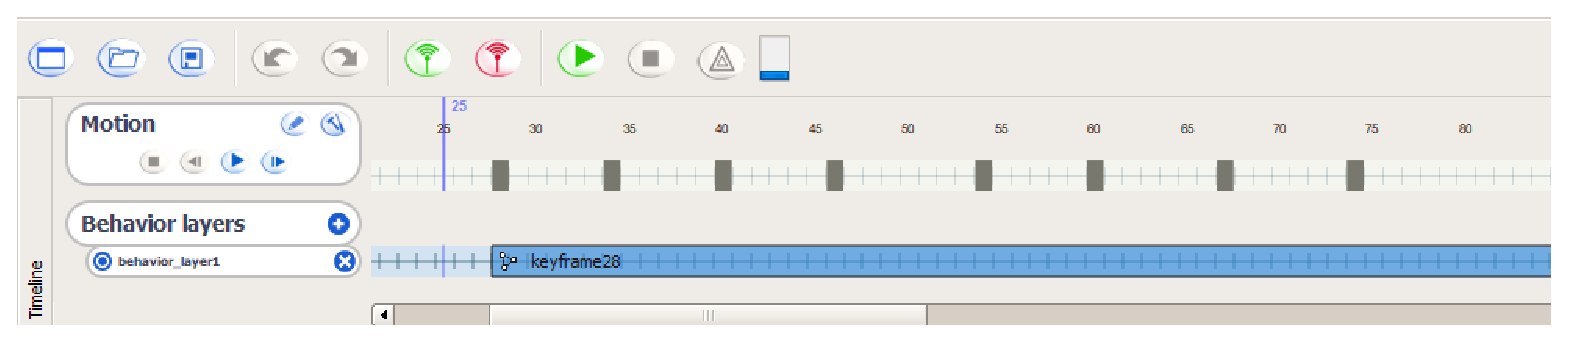
\includegraphics[width=0.75\textwidth,height=0.75\textheight,keepaspectratio]{timeline}
  \caption{The timeline feature in Choregraphe.}
	\label{fig:timeline}
\end{figure}

As some more complicated animations are harder to create on the virtual robot, animating hands-on with the NAO robot can also be done. This is usually easier with two people, where one person manipulates the robot, and another stands by the computer to save postures into keyframes. This way, the process is usually something as follows:
\begin{enumerate}
	\item {Assume Person A is by the computer, and Person B is by the robot.}
	\item {Person A loosens the limbs that are to be animated, using the "Stiffen chain" button as shown in Figure \ref{fig:choregraphe-movement}.}
	\item{Person B manipulates the robot to the desired position.}
	\item{Person A stores the position data to a keyframe at a desired place in the timeline.}
	\item{Repeat.}
\end{enumerate}
This is the process that we used for movements such as pointing at a leg, or mimicking a car crash with the robot's hands.
By organizing certain movements into separate boxes, it is also easier to copy and paste certain motions.
Because of the nature of Choregraphe's behavior when saving positions, the animators should be wary of which limbs are being saved.
While only a few select limbs may be used for animation, storing all of the robot's limbs positions may yield unexpected results when paired with a preceding or proceeding animation that involves separate limbs. It is usually best to only store the position of the limbs that are intended to move, to prevent knee-jerk reactions from the robot.



\subsection{Designing a Performance}

    \subsubsection{The Room}
    The comedian will have a better performance if the crowd is in a more comfortable space.
    For the 2018 Engineering Expo, we requested a closed room, with seats, and plenty of room to stand.
    The needs of the crowd is dependent on the audience you are trying to reach during the show.


    The only reason we had standing room is because we didn't have enough seats, and some people only wanted to see the show and not participate.
    This was also the only place at the engineering expo with a place to sit.
    People are comfortable when they are sitting.
    We could have made this better by making the room dark, and putting the lights on the robot.
    \subsubsection{The Seed}
    This is where Ginger would ask the audience what kind of show they would like to hear, either "Jobs, Aging, or Romance".
    It is generally not advised to ask the audience what they want, as it is the job of the comedian tell their best jokes.


    By branching based on the majority of the responses, it was difficult to give everyone what they wanted, therefore dividing the crowd.
    The crowd needs to feel like they are together, laughing at the same thing.
    When we branched between shows, there often wasn't very high audience participation.
    If the audience is loosing interest, it is \textbf{essential} to run a Crowd Work Routine, to get the audience paying attention to the robot.
    \subsubsection{The Middle Part}

    After performing crowdwork, the audience should be setup for a comedy show. This is where we implemented most of jokes that we had written.
    We knew Ginger could perform about 5 minutes of Comedy, so we had the robot tell 4 jokes from the topic that was branched to during the Seed portion of the show.
    Since we had the same 4 jokes that had modified setups (depending on the branched topic), it is better to find the best version of a single joke, and tell the audience that version. We found that it was better tell our better jokes during the beginning, as the audience was hooked into the rest of the set.

    We used the NAO microphones to collect audio information, and correlate that to the behavior of the current running joke.
    If the crowd was louder during the middle of a joke, they often could not hear the end of the joke.
    It is better to use external recording, and then give the simple response back to the robot.

    \subsubsection{Ending the Show}

    This is when the Robot is out of jokes, and needs to end the show.
    For comedy, it is a good idea to end the show quickly, so that the audience wants more from the show.

    This is where we implemented the "Crowd Report", that told the audience how the robot thought the show went.
    The Crowd Report was intended to collect information during the show, and present the robot's insinuations about the crowd back.
    A common, written, response on the survey question "What did you find was surprising about the show?" was that most people did not know that the robot was collecting data on the crowd.


    Not storing information about the show could make the crowd feel more comfortable.


\subsection{Audience Input}
    We tried using two methods of audience input: Microphone Decibel Level, and Hand Held Controllers.
    These two methods are ineffective at collecting data, as the crowd did not know how to interact with the robot.
    The crowd should instead be instructed, as simply as possible, how to interact with the robot.


    The Microphone Decibel level was poor at receiving information because the mic was centered on the robots head.
    Using decibel level alone, the microphone was unable to distinguish between booing and cheering.
    Additionally, clapping was significantly louder than laughing.
    If one person clapped in the front, the response (according to the robot), was louder than if the whole crowd was listening.
    It is more effective if there are multiple microphones distributed around the room.


    We also tried using controllers with buttons to receive audience input.
    This was ineffective, because when the crowd was given the controllers, the focus was taken off of the robot.
    The audience should only be listening to the robot, and not paying attention to the controllers in their hands.
    More work should be done to investigate how to model a physical audience into a virtual audience for the robot.

\subsection{Technical Resources}

    The NAOqi API was challenging to work with. The documentation is scarce, all over the place, and often outdated.
    Some of the example code is in C++, while some is in Python. Also, there are two versions of the NAOqi SDK, both of which seem to be intercompatible.
    This makes it hard to interpret what each of the functions do.
    However, using it is the only way to operate the robot without using the clunky Choregrahe GUI.
    The NAOqi API came particularly handy during the shows and helped launch behaviors without much delay, unlike Choregraphe.

    Setting up the NAOqi SDK was a doozy in itself. For setting it up on a Mac, it needs to run on the built-in Python version,
    NOT the one from the official Python website. This is fine, but it does not work with the built-in Python version on the latest versions of OS X.
    I understand that this is due to the security measures in the newer versions of OS X, but the documentation hasn't been updated to reflect that.
    While not knowing this, and trying to get around it took a while, there is a Bash script \cite{BashScript}
    that "fixes" the Python installation to match the NAOqi requirements.

    There are similar issues with the NAOqi SDK on Ubuntu 16.04 (and probably other versions as well). StackOverflow had some takes
    on what could fix the issue \cite{naoUbuntu}. It involved modifying some of the installation files as well.

    Once all of that is set up, the documentation provided on the Aldebaran website \cite{AldebaranDoc} has some example code for various different functionalities on the robot.
    As mentioned earlier, some of the documentation is in C++ and some of the documentation from the older NAOqi version is intercompatible as well.
    This requires some trial and error to see what function calls work with Python.
